%%% Template originaly created by Karol Kozioł (mail@karol-koziol.net) and modified for ShareLaTeX use

\documentclass[a4paper,11pt]{article}

\usepackage[T1]{fontenc}
\usepackage[utf8]{inputenc}
\usepackage{graphicx}
\usepackage{xcolor}
\usepackage[export]{adjustbox}
\usepackage{titlesec}
\usepackage{sectsty}
\allsectionsfont{\sffamily}
\usepackage{microtype}
\usepackage{tgheros}
\usepackage{droidsansmono}
\usepackage{mathptmx}
\usepackage{lastpage}
\usepackage{amsmath,amssymb,amsthm,textcomp}
\usepackage{enumerate}
\usepackage{multicol}
\usepackage{tikz}
\usepackage{tabto}
\usepackage{pxfonts}
\usepackage{geometry}
\geometry{left=25mm,right=25mm,%
bindingoffset=0mm, top=20mm,bottom=20mm}


\linespread{1.2}
\makeatletter
\renewcommand\tableofcontents{%
    \section*{\makebox[\linewidth][c]{\contentsname}%
      \@mkboth{\MakeUppercase\contentsname}{\MakeUppercase\contentsname}}%
    \begin{multicols}{2}%
    \@starttoc{toc}%
    \end{multicols}
    }
\makeatother
\newcommand{\linia}{\rule{\linewidth}{0.5pt}}

% custom theorems if needed
\newtheoremstyle{mytheor}
    {1ex}{1ex}{\normalfont}{0pt}{\scshape}{.}{1ex}
    {{\thmname{#1 }}{\thmnumber{#2}}{\thmnote{ (#3)}}}

\theoremstyle{mytheor}
\newtheorem{defi}{Definition}
\newtheoremstyle{mytheor}
    {1ex}{1ex}{\normalfont}{0pt}{\scshape}{|}{1ex}
    {{\thmname{#1 }}{}{\thmnote{ (#3)}}}

\theoremstyle{mytheor}
\newtheorem{nb}{Please Note}
% my own titles
\makeatletter
\renewcommand{\maketitle}{
\begin{center}
\vspace{2ex}
{\huge \textsf{\textbf{\@title}}}
\vspace{1ex}
\\
\linia\\
\textsf{\@date \hfill
\@author}
\vspace{4ex}
\end{center}
}
\makeatother
%%%
\usepackage{array}

% custom footers and headers
\usepackage{fancyhdr}
\pagestyle{fancy}
\lhead{}
\chead{}
\rhead{}
\lfoot{Assignment 4}
\cfoot{}
\rfoot{Page \thepage \ of \pageref{LastPage}}
\renewcommand{\headrulewidth}{0pt}
\renewcommand{\footrulewidth}{0pt}
%

% code listing settings
\usepackage{listings}
\usepackage[space=true]{accsupp}
\newcommand{\noncopynumber}[1]{
    \BeginAccSupp{method=escape,ActualText={}}
    #1
    \EndAccSupp{}
}
\definecolor{codegreen}{rgb}{0,0.6,0}
\definecolor{codegray}{rgb}{0.5,0.5,0.5}
\definecolor{inlinecode}{rgb}{0.1,0.1,0.1}
\definecolor{codepurple}{rgb}{0.58,0,0.82}
\definecolor{backcolour}{rgb}{0.95,0.95,0.92}
\lstset{
    language=C,
    basicstyle=\ttfamily\small,
    aboveskip={1.0\baselineskip},
    breakatwhitespace=false,         
    keepspaces=true,
    belowskip={1.0\baselineskip},
    columns=fullflexible,
    extendedchars=true,
    breaklines=true,
    tabsize=4,
    frame=lines,
    showtabs=false,
    showspaces=false,
    showstringspaces=false,
    commentstyle=\color{codegray},
    keywordstyle=\bfseries,
    %stringstyle=\rmfamily,
    numbers=left,
    numberstyle=\color{codegray}\footnotesize\noncopynumber,
    stepnumber=1,
    numbersep=10pt,
    captionpos=t,
    escapeinside={\%*}{*)},
}


\lstdefinestyle{output}{
    basicstyle=\ttfamily\small,
    aboveskip={1.0\baselineskip},
    breakatwhitespace=false,         
    keepspaces=true,
    belowskip={1.0\baselineskip},
    columns=fullflexible,
    extendedchars=true,
    breaklines=true,
    tabsize=4,
    frame=lines,
    showtabs=false,
    showspaces=false,
    showstringspaces=false,
    captionpos=t
}
%%%----------%%%----------%%%----------%%%----------%%%

\begin{document}

\title{CSE-016 Programming Lab Assignment \textnumero{} 4}

\date{22/04/2024}

\author{Youssef Ahmed Samy Kassem\\ \hfill ID 9545 -- Group 3 -- Lab 1\\ \hfill SSP -- Faculty of Engineering, Alexandria University\\}

\maketitle
\textsf{\textsl{\textbf{Solutions begin from the second page.}}}
\section{Problems}
\subsection{Problem (1)}
Write a program to determine whether a given number is prime or not.\\
\textbf{\underline{Example 1:}}\\
Enter a number: 13\\
13 is a prime number\\
\textbf{\underline{Example 1:}}\\
Enter a number: 28\\
28 is not a prime number
\subsection{Problem (2)}
Write a program that uses looping to print the following table of values.\\

\includegraphics[width=0.5\linewidth]{image.png}
\tableofcontents
\newpage
\section{Solutions}
\subsection{Solution to Problem (1)}
\subsubsection{Source Code}
\begin{lstlisting}[escapechar=\^,label={list:first},title=Program's \texttt{C} code | Line numbers for readability]
#include <stdio.h>
int main()
{
    int num, is_prime = 1, counter;
    printf("Enter a number: ");
    scanf("%d", &num);
    if (num < 2 || (num > 2 && num % 2 == 0))
    {
        is_prime = 0;
    } else {
        for (counter = 3; counter < num; counter = counter + 2)
        {
            if (num % counter == 0) { is_prime = 0; break; }
        }
    }
    if (is_prime)
    {
        printf("%d is a prime number\n", num);
    } else {
        printf("%d is not a prime number\n", num);
    }
    return 0;
}
\end{lstlisting}
\begin{nb}
    0 \& 1 are not considered prime numbers by most contemporary mathematicians.
\end{nb}
\subsubsection{Outcome}
\paragraph{Console Output}
\begin{lstlisting}[escapechar=\%,style=output,numbers=none,label={list:second},title=Program's output to console in plaintext -- \texttt{13} as input]
Enter a number: 13
13 is a prime number
%
\end{lstlisting}
\begin{lstlisting}[escapechar=\%,style=output,numbers=none,label={list:second-second},title=Program's output to console in plaintext -- \texttt{28} as input]
Enter a number: 28
28 is not a prime number
%
\end{lstlisting}
\subsection{Solution to Problem (2)}
\subsubsection{Source Code}
\begin{lstlisting}[label={list:third},title=Program's \texttt{C} code -- uses \texttt{for} loop to print out table | Line numbers for readability]
#include <stdio.h>

int main()
{
    int n;
    printf("N\t10*N\t100*N\t1000*N\n\n");
    for (n=1; n<=10; n++)
    {
        printf("%d\t%d\t%d\t%d\n", n, n*10, n*100, n*1000);
    }
    return 0;
}
\end{lstlisting}
\subsubsection{Outcome}
\paragraph{Console Output}
\begin{lstlisting}[escapechar=\%,style=output,numbers=none,label={list:fourth},title=Program's output to console in plaintext]
N       10*N    100*N   1000*N

1       10      100     1000
2       20      200     2000
3       30      300     3000
4       40      400     4000
5       50      500     5000
6       60      600     6000
7       70      700     7000
8       80      800     8000
9       90      900     9000
10      100     1000    10000
%
\end{lstlisting}
\newpage
\subsection{Evidence of Work (Screenshots)}
\begin{figure}[!h]
    \centering
    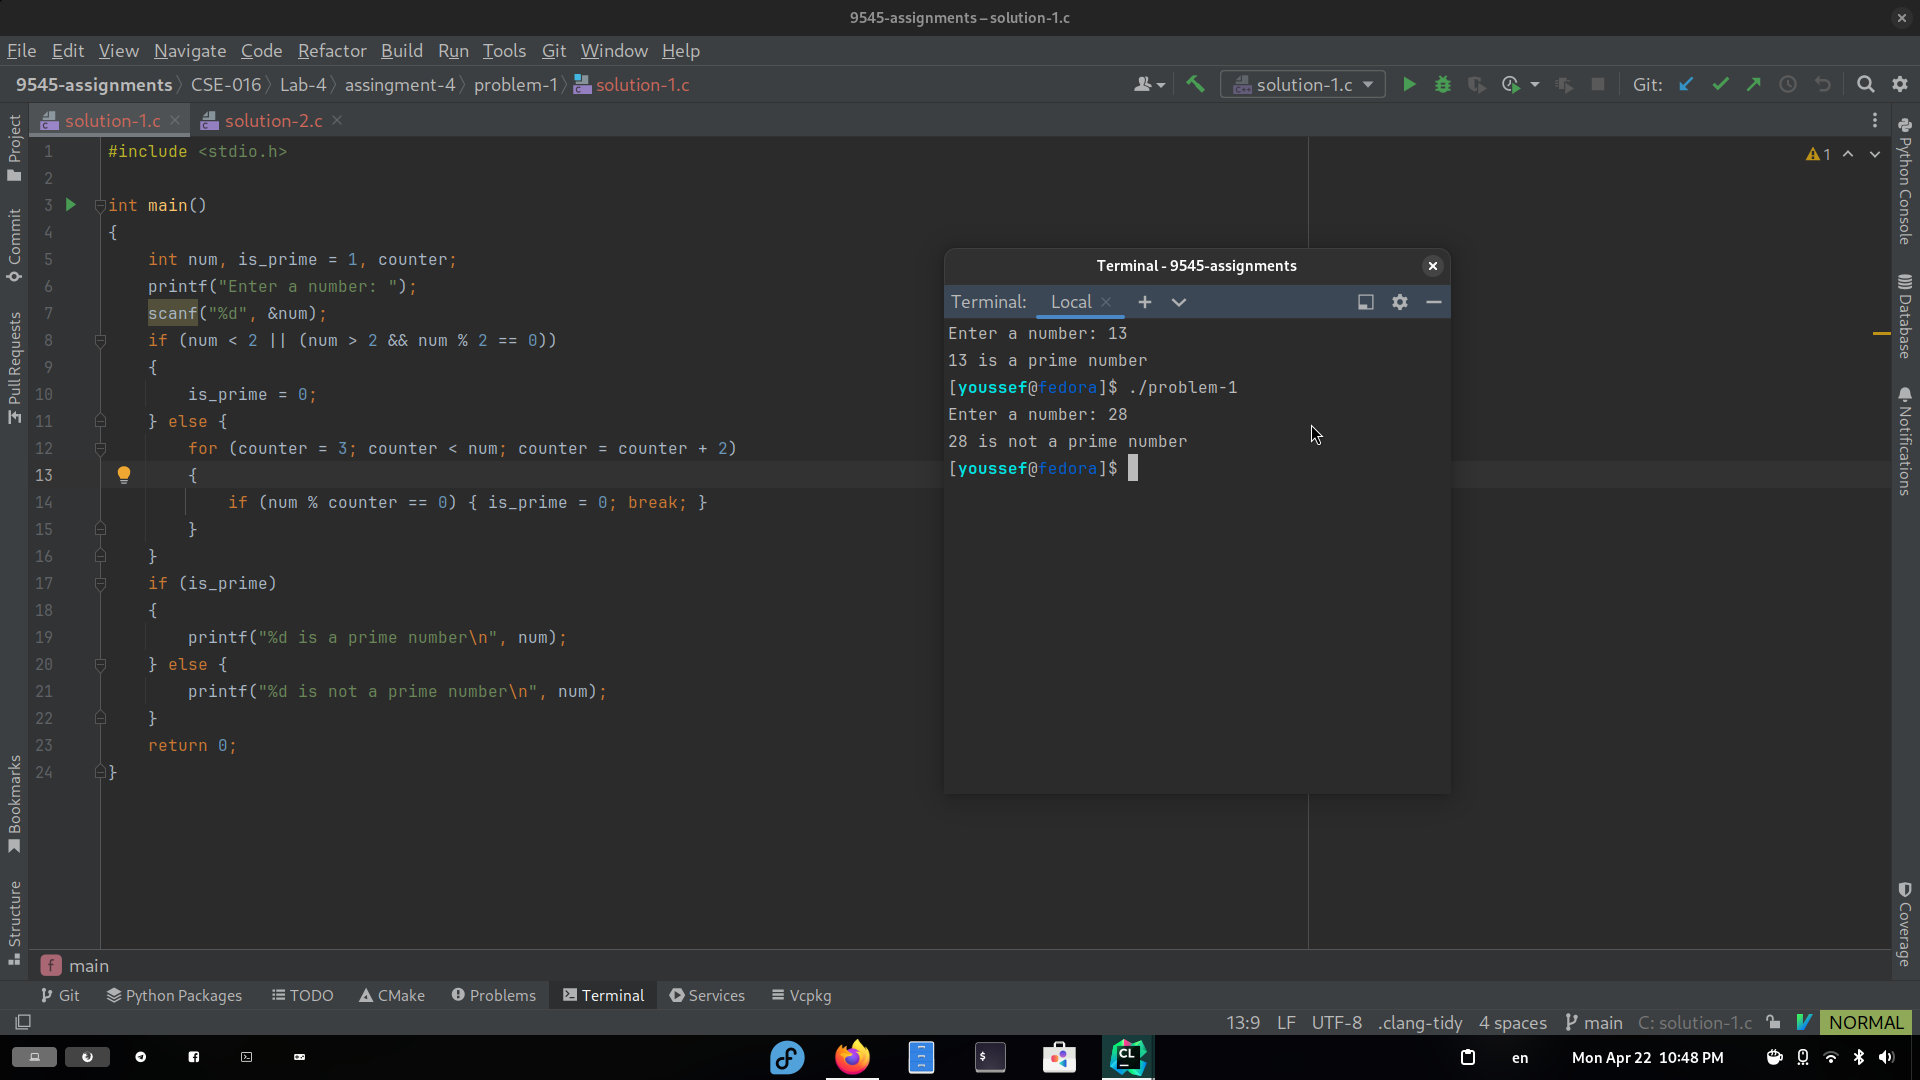
\includegraphics[width=\linewidth]{prob-1.png}
    \caption{Desktop screenshot of Problem (1)'s code in CLion}
\end{figure}
\begin{figure}[!h]
    \centering
    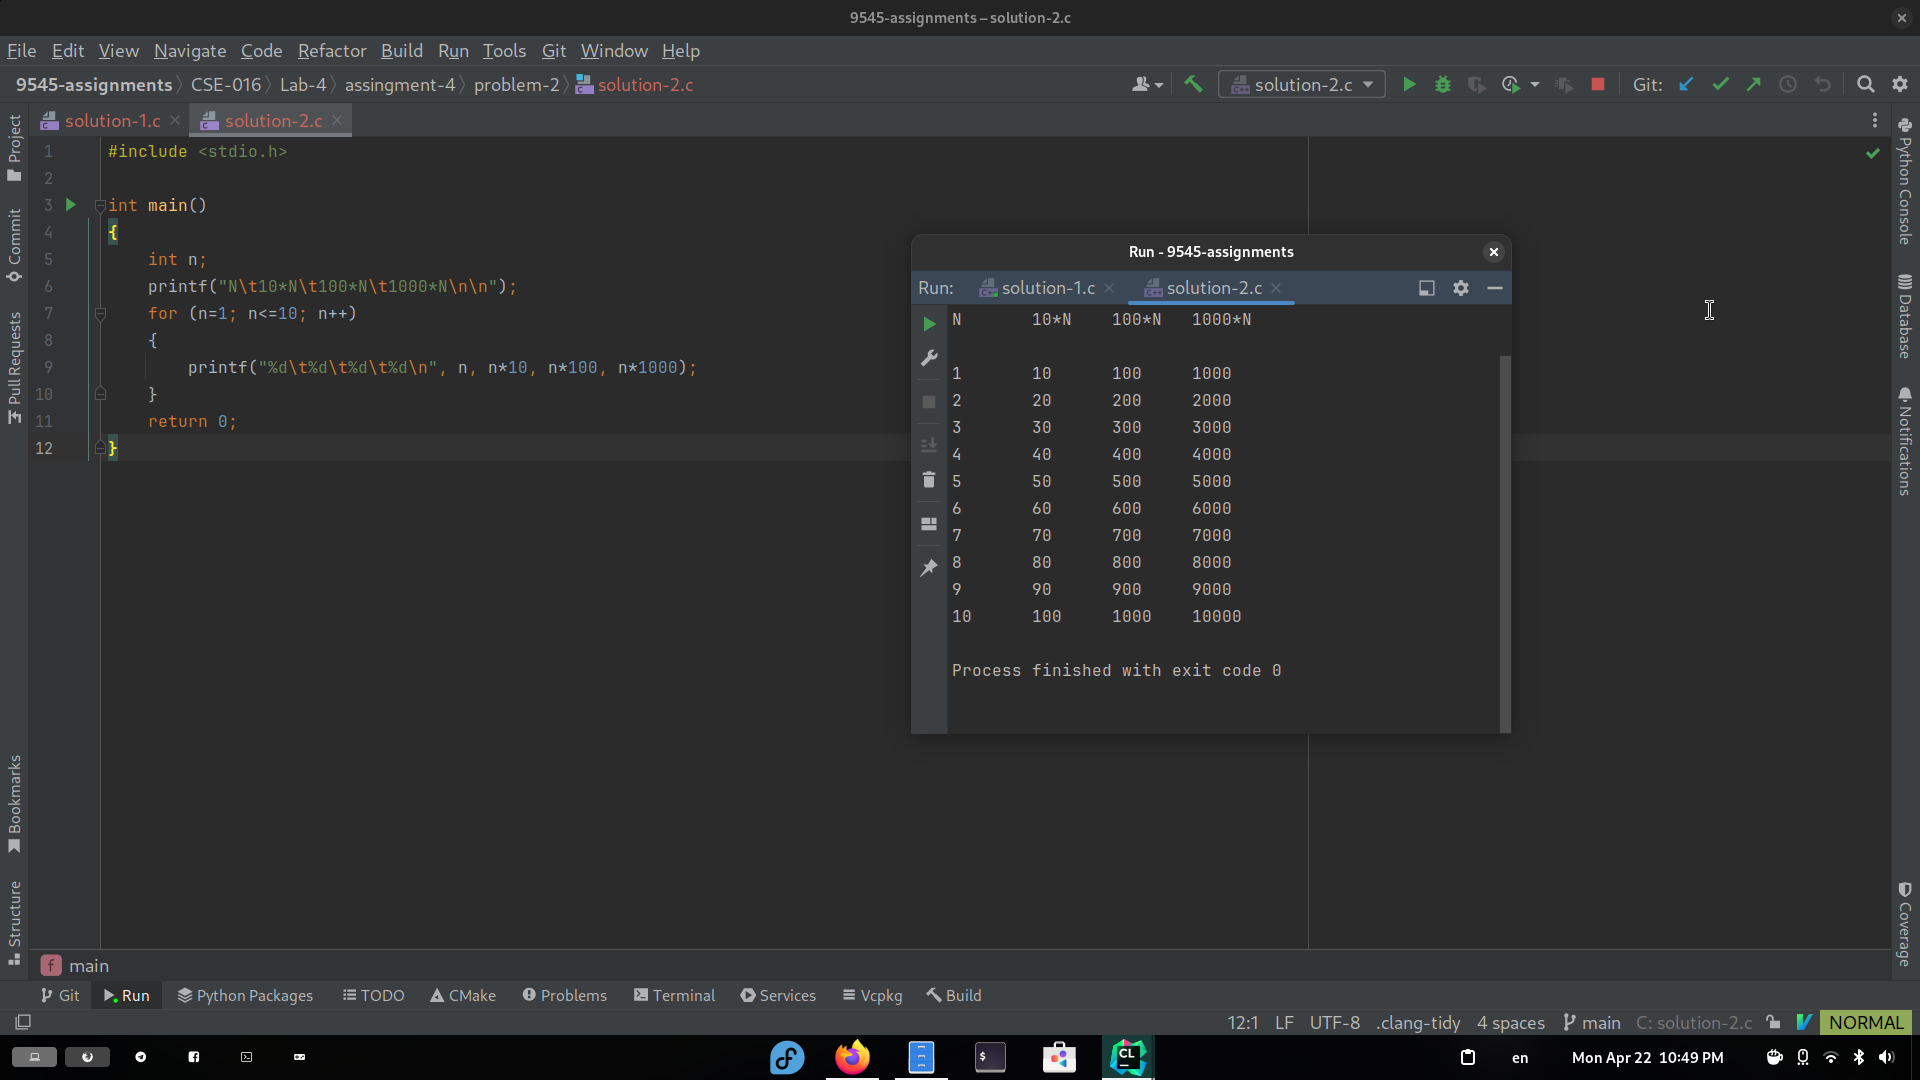
\includegraphics[width=\linewidth]{prob-2.png}
    \caption{Desktop screenshot of Problem (2)'s code in CLion}
\end{figure}
\newpage
\subsection{Specifications}
\begin{itemize}
    \item \textbf{Libraries:}
    \begin{itemize}
        \item \texttt{\color{inlinecode}{stdio.h}}
    \end{itemize}
    \item \textbf{Compiler:} GNU C Compiler \texttt{\color{inlinecode}{(gcc)}} version 14.0.1 20240328 (Red Hat 14.0.1-0)
    \item \textbf{C Standard Compatibility}
    \begin{center}
        \begin{tabular}{|c|c|c|c|c|c|}
             \hline
             \textbf{P\#} & \textbf{C89/C90} & \textbf{C99} & \textbf{C11} & \textbf{C17} & \textbf{C23} \\
             \hline
              1 & \checkmark & \checkmark & \checkmark & \checkmark & \checkmark \\
              2 & \checkmark & \checkmark & \checkmark & \checkmark & \checkmark \\
             \hline
        \end{tabular}
    \end{center}
    
    %\begin{flushright}
    %    \begin{tabular}{c|c}
    %         Symbol & Compatibility  \\
    %         \hline
    %         \checkmark & Full \\
    %         $\sim$ & Non-Fatal Errors \\
    %         $\times$ & Incompatible
    %    \end{tabular}
    %\end{flushright}
    \item \textbf{Supported Platforms:} OS: (any), architecture: (any)
    \item \textbf{Tested On:} Fedora 40 Workstation Linux
\end{itemize}
\section{Licenses}
This document, my additions to its \LaTeX \ source code, the software included and its \texttt{C} source code all come without warranty and are all subject to the BSD 3-Clause Open Source License:\\https://opensource.org/license/bsd-3-clause.\\

\begin{center}
    COPYRIGHT \copyright \ 2024, Youssef Ahmed Samy
\end{center}
\fancypagestyle{lastpage}
{
   \fancyhf{}
   \fancyfoot[C]{\textsl{END OF DOCUMENT}}
   \fancyfoot[L]{Assignment 4}
    \rfoot{Page \thepage \ of \pageref{LastPage}}
}
\thispagestyle{lastpage}
\end{document}
